\section{Wasserdargebot für Wasserkraft}

\subsection{Abflussganglinie}
    \begin{minipage}[t]{0.4\columnwidth}
        Abfluss $Q_b$ in \unit{\cubic\metre\per\second} während eines Jahres (365 Tage)
    \end{minipage}%
    \hfill
    \begin{minipage}[c]{0.58\columnwidth}
        \begin{center}
            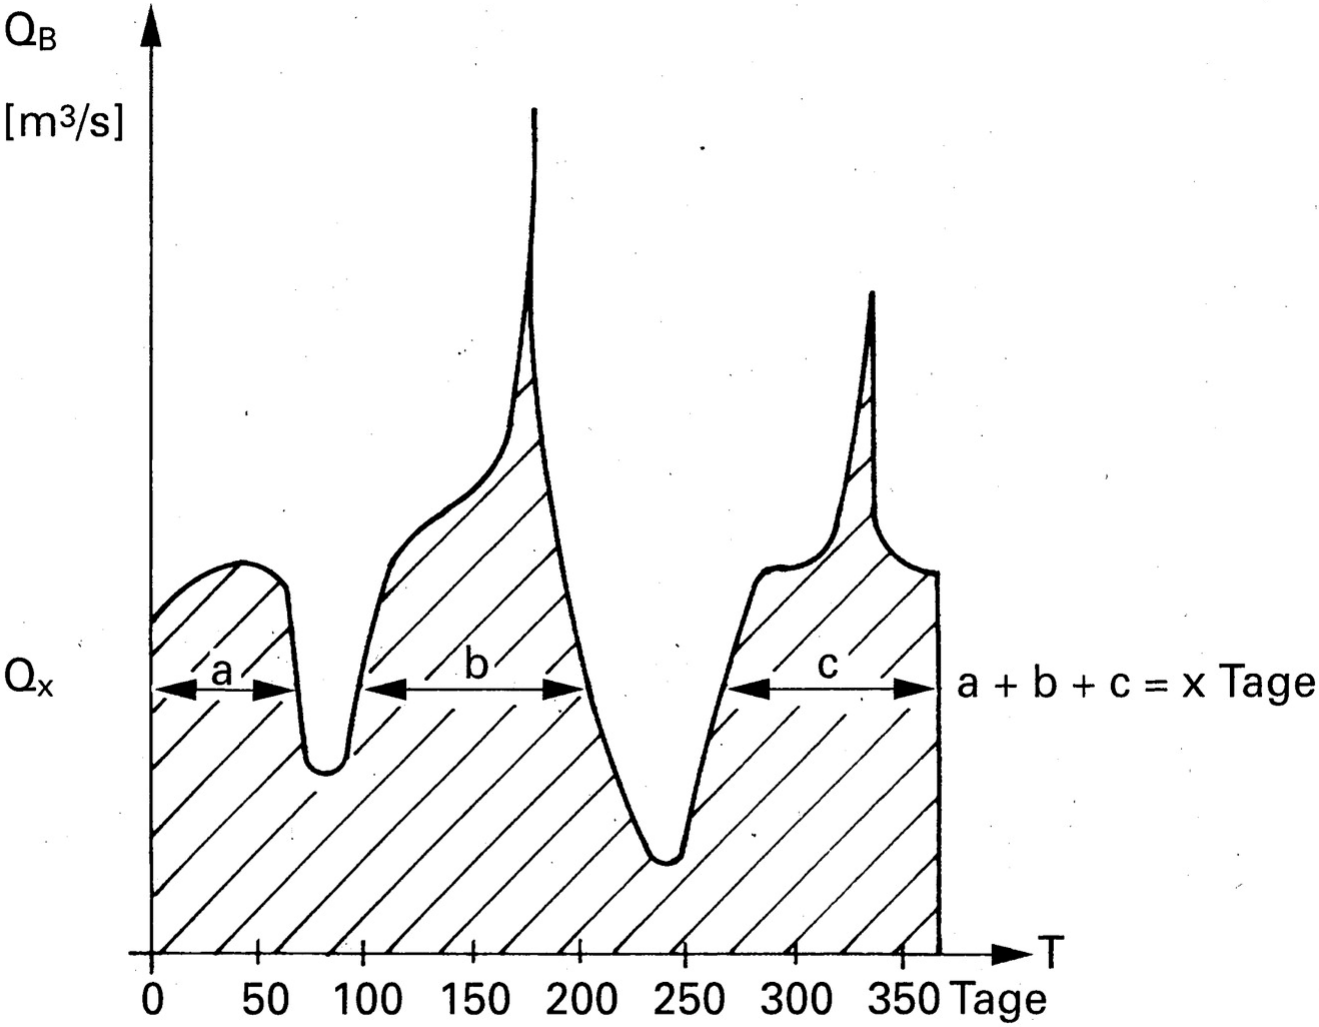
\includegraphics[width=0.95\textwidth, align=c]{images/Abflussganglinie.png}
        \end{center}
    \end{minipage}

\subsection{Abflussdauerkurve}
    \begin{minipage}[t]{0.4\columnwidth}
        Abfluss $Q_b$ in \unit{\cubic\metre\per\second} während eines Jahres (365 Tage), sortiert der Grösse nach

        \medskip

        \textbf{Abfluss ist an 275 Tagen mindestens $Q_x$}
    \end{minipage}%
    \hfill
    \begin{minipage}[c]{0.48\columnwidth}
        \begin{center}
            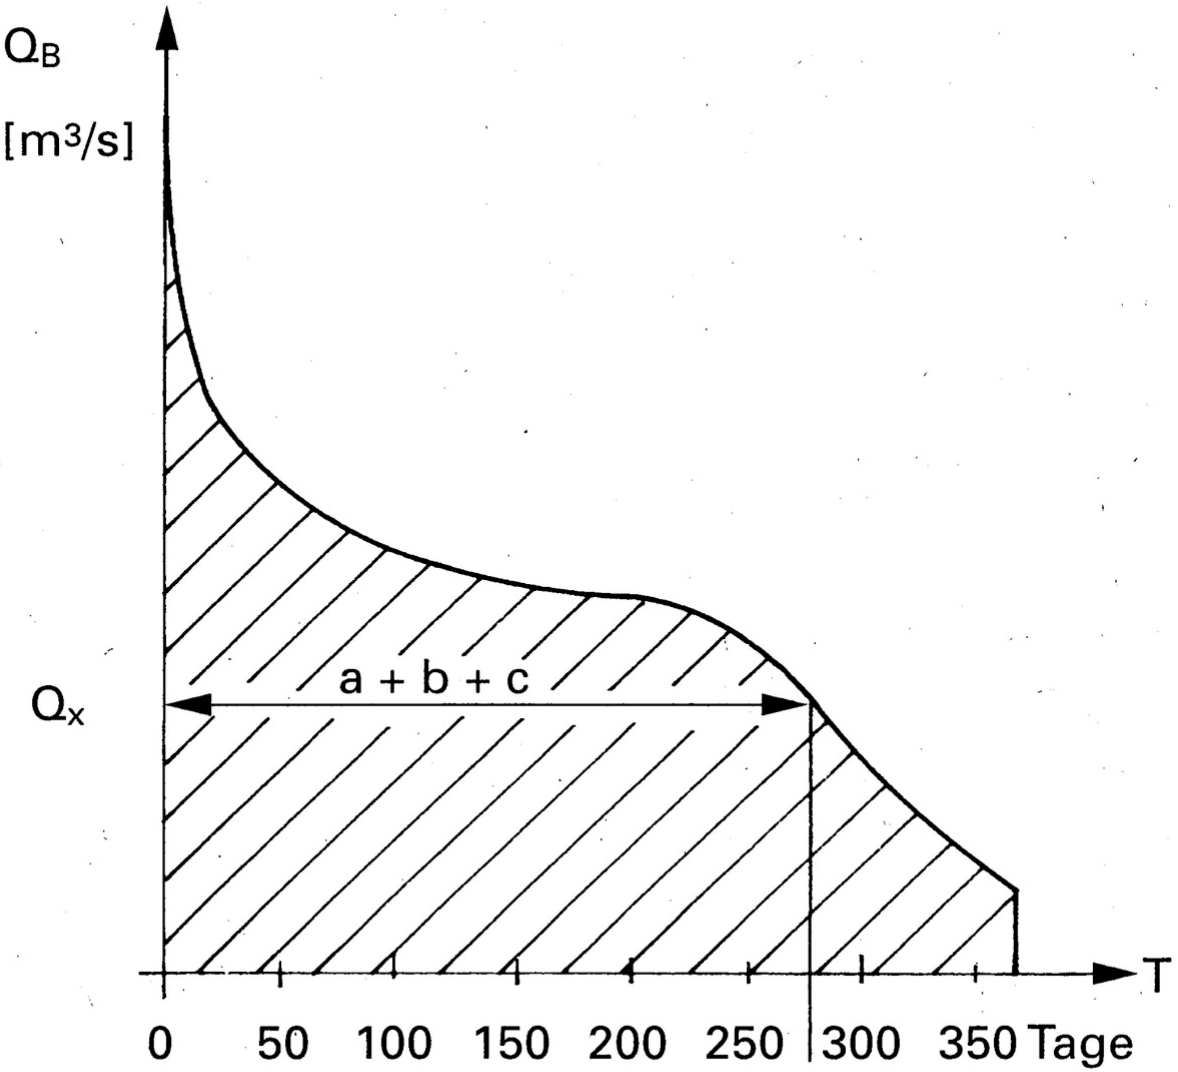
\includegraphics[width=0.95\textwidth, align=c]{images/Abflussdauerkurve.png}
        \end{center}
    \end{minipage}

\subsection{Nutzwassermenge}
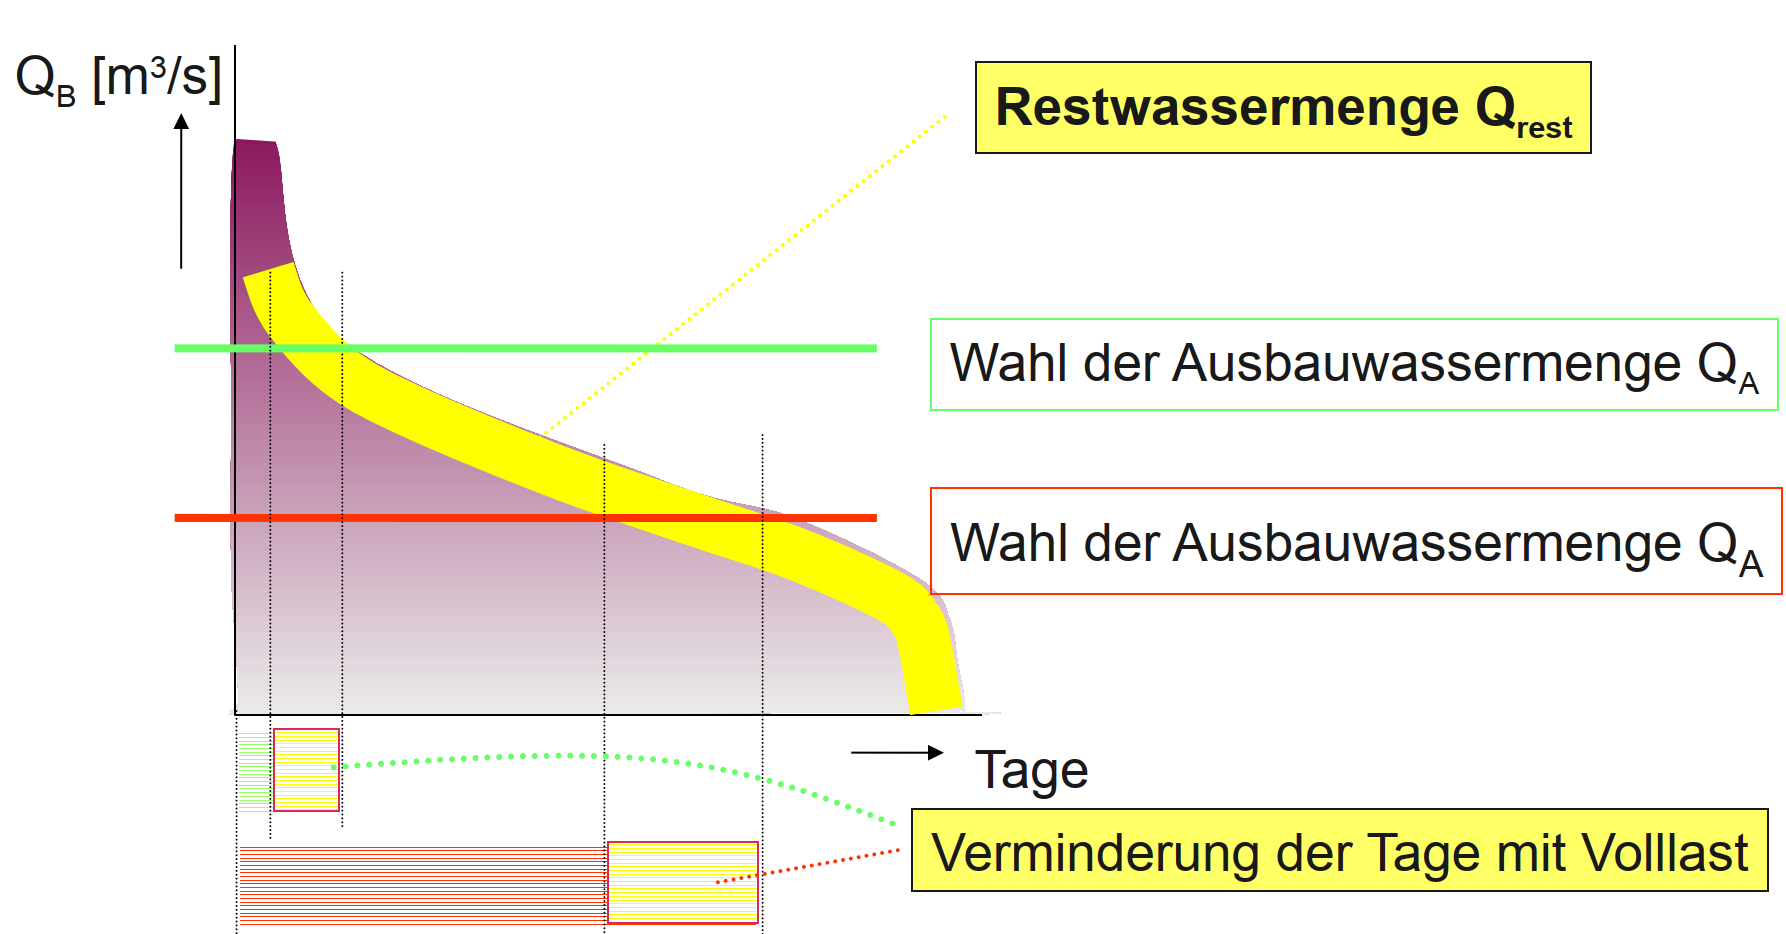
\includegraphics[width=0.8\columnwidth, align=c]{images/Nutzwassermenge.png}

\vspace{0.1cm}

$\boxed{Q_{Nutz} = Q_B - Q_{Rest}}$

\vspace{0.1cm}

\renewcommand{\arraystretch}{1.2} % Erhöht Zeilenhöhe für bessere Lesbarkeit
\begin{tabular}{@{} l p {6cm} l @{}}
    $[Q_{Nutz}]$    & Nutzwassermenge   \dotfill & \unit{\cubic\metre\per\second} \\
    $[Q_B]$         & Abflussmenge      \dotfill & \unit{\cubic\metre\per\second} \\
    $[Q_{Rest}]$    & Restwassermenge   \dotfill & \unit{\cubic\metre\per\second} \\
\end{tabular}

\subsubsection{Mindest Restwassermenge $Q_{\mathrm{Rest}}$}

$Q_{\mathrm{Rest}}$ muss aufgrund von ökologischen Mindestanforderungen \textbf{immer} gewährleistet sein.

\begin{tabular}{>{\raggedright}p{6.5cm} r}
\toprule
\textbf{Abflussmenge $Q_{347}$} & \textbf{Restwassermenge} \\
\midrule
bis 60 l/s Abflussmenge $Q_{347}$ & 50 l/s \\
$\to$ pro weitere 10 l/s Abflussmenge $Q_{347}$ & 8 l/s mehr \\
\addlinespace
bis 160 l/s Abflussmenge $Q_{347}$ & 130 l/s \\
$\to$ pro weitere 10 l/s Abflussmenge $Q_{347}$ & 4{,}4 l/s mehr \\
\addlinespace
bis 500 l/s Abflussmenge $Q_{347}$ & 280 l/s \\
$\to$ pro weitere 100 l/s Abflussmenge $Q_{347}$ & 31 l/s mehr \\
\addlinespace
bis 2500 l/s Abflussmenge $Q_{347}$ & 900 l/s \\
$\to$ pro weitere 100 l/s Abflussmenge $Q_{347}$ & 21{,}3 l/s mehr \\
\addlinespace
bis 10\,000 l/s Abflussmenge $Q_{347}$ & 2\,500 l/s \\
$\to$ pro weitere 1\,000 l/s Abflussmenge $Q_{347}$ & 150 l/s mehr \\
\addlinespace
ab 60\,000 l/s Abflussmenge $Q_{347}$ & 10\,000 l/s \\
\bottomrule
\end{tabular}

\subsection{Triebwassersystem}
Ein Triebwassersystem führt das Wasser vom Speicher zur Turbine eines Wasserkraftwerks. 
Es beinhaltet die Leitungswege wie Stollen und Druckleitungen. 
Verluste darin sind bei Speicherkraftwerken bedeutsam, bei Laufwasserkraftwerken jedoch meist vernachlässigbar.